\section{Search for a Kinematic Edge}
\label{sec:fit}

We search for a kinematic edge in the dilepton mass distribution. Such a feature is 
predicted to occur in SUSY models in which the opposite-sign leptons are produced by the
decay $\chi_2^0 \to \chi_1^0 \ell^+\ell^-$. Such models tend to produce an excess of pairs 
of same-flavor (SF) $ee$ or $\mu\mu$ leptons with respect to opposite-flavor (OF) $e\mu$
leptons; hence we search for this kinematic edge in events containing SF lepton pairs. 
For the \ttbar\ background, the rates of SF and OF lepton pairs are the same;
furthermore, the kinematic properties of events containing SF and DF lepton pairs are the
same. Thus we can extract the shape of the \ttbar\ dilepton mass distribution from events 
containing OF leptons, and apply it to events containing SF leptons.

In order to further suppress DY, we increase the \MET\ requirement to \MET $>$ 100 GeV. 
We search for the kinematic edge in 2 regions.  The first region is a control region defined
as 100 $<$ \Ht\ $<$ 300 GeV, which is expected to be dominated by the \ttbar\ background; we use 
this region to validate our fit methodology and verify that a signal yield consistent with 0 
is obtained. We then proceed to search for a kinematic edge in the signal region defined as 
\Ht\ $>$ 300 GeV. Since we do not observe a kinematic edge in this region, we perform a 
fit to the dilepton mass distribution assuming an example signal shape from the LM1 scenario.

For each region, we begin by extracting the \ttbar\ shape from the dilepton mass distribution 
in events containing OF lepton pairs, as shown in Fig.~\ref{fig:dilmasscontrol} (right). 
The background is described by:

\begin{equation}
B(\mll) = \mll^a e^{-b \mll}.
\end{equation}

For a potential signal, we use an edge model for a two-body decay, which comprises a triangular shape convoluted with a gaussian,
according to:

\begin{equation}
T(\mll) = \frac{1}{\sqrt{2\pi}\sigma}\int_0^{M_{cut}} dy~y e^{\frac{(-(\mll-y)^2}{2\sigma^2}}. 
\end{equation}


\begin{figure}[tbh]
\begin{center}
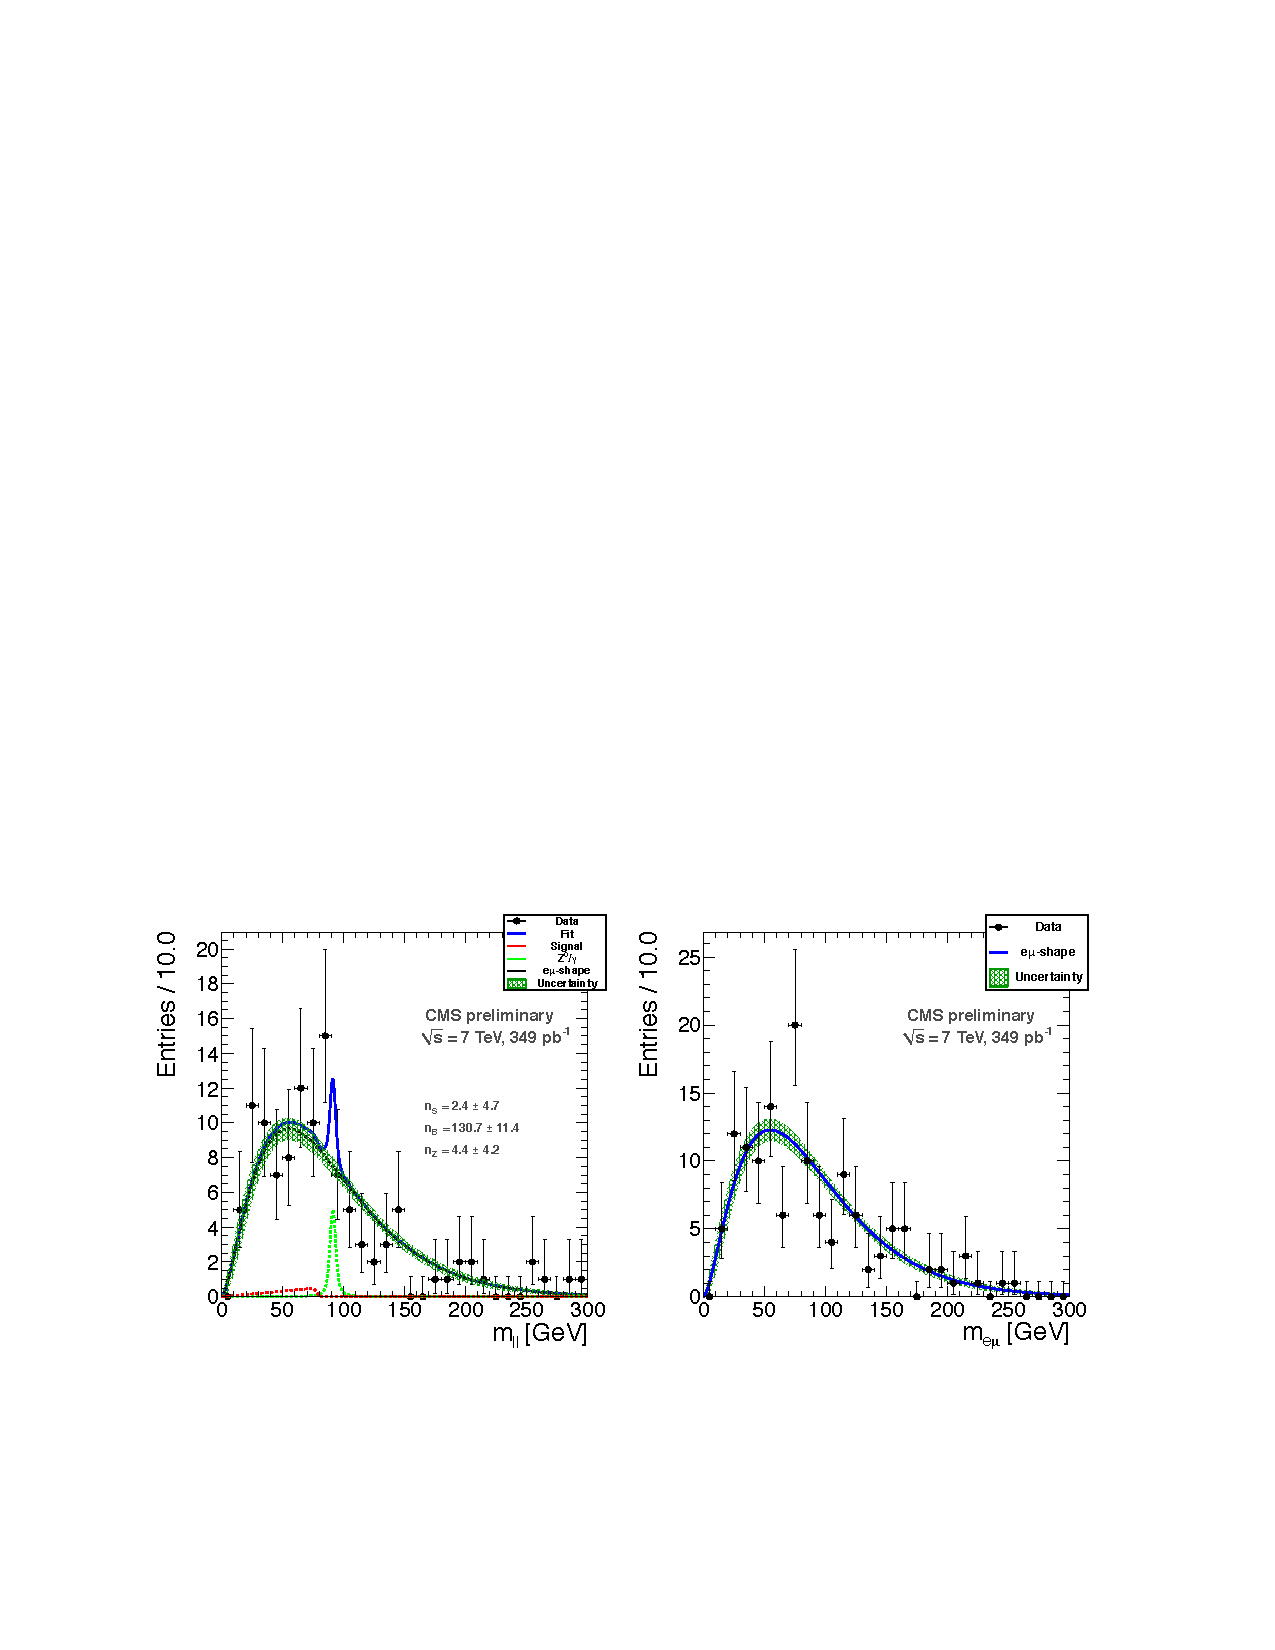
\includegraphics[width=0.75\linewidth]{plots_final/dilmass_control.pdf}
\caption{\label{fig:dilmasscontrol}\protect 
Results of the maximum likelihood fit to the dilepton mass distribution for events containing 
$ee$ and $\mu\mu$ lepton pairs (left) and $e\mu$ lepton pairs (right) in the control
region defined as 100 $<$ \Ht\ $<$ 300~GeV, \MET\ $>$ 100 GeV.
}
\end{center}
\end{figure}

\begin{figure}[tbh]
\begin{center}
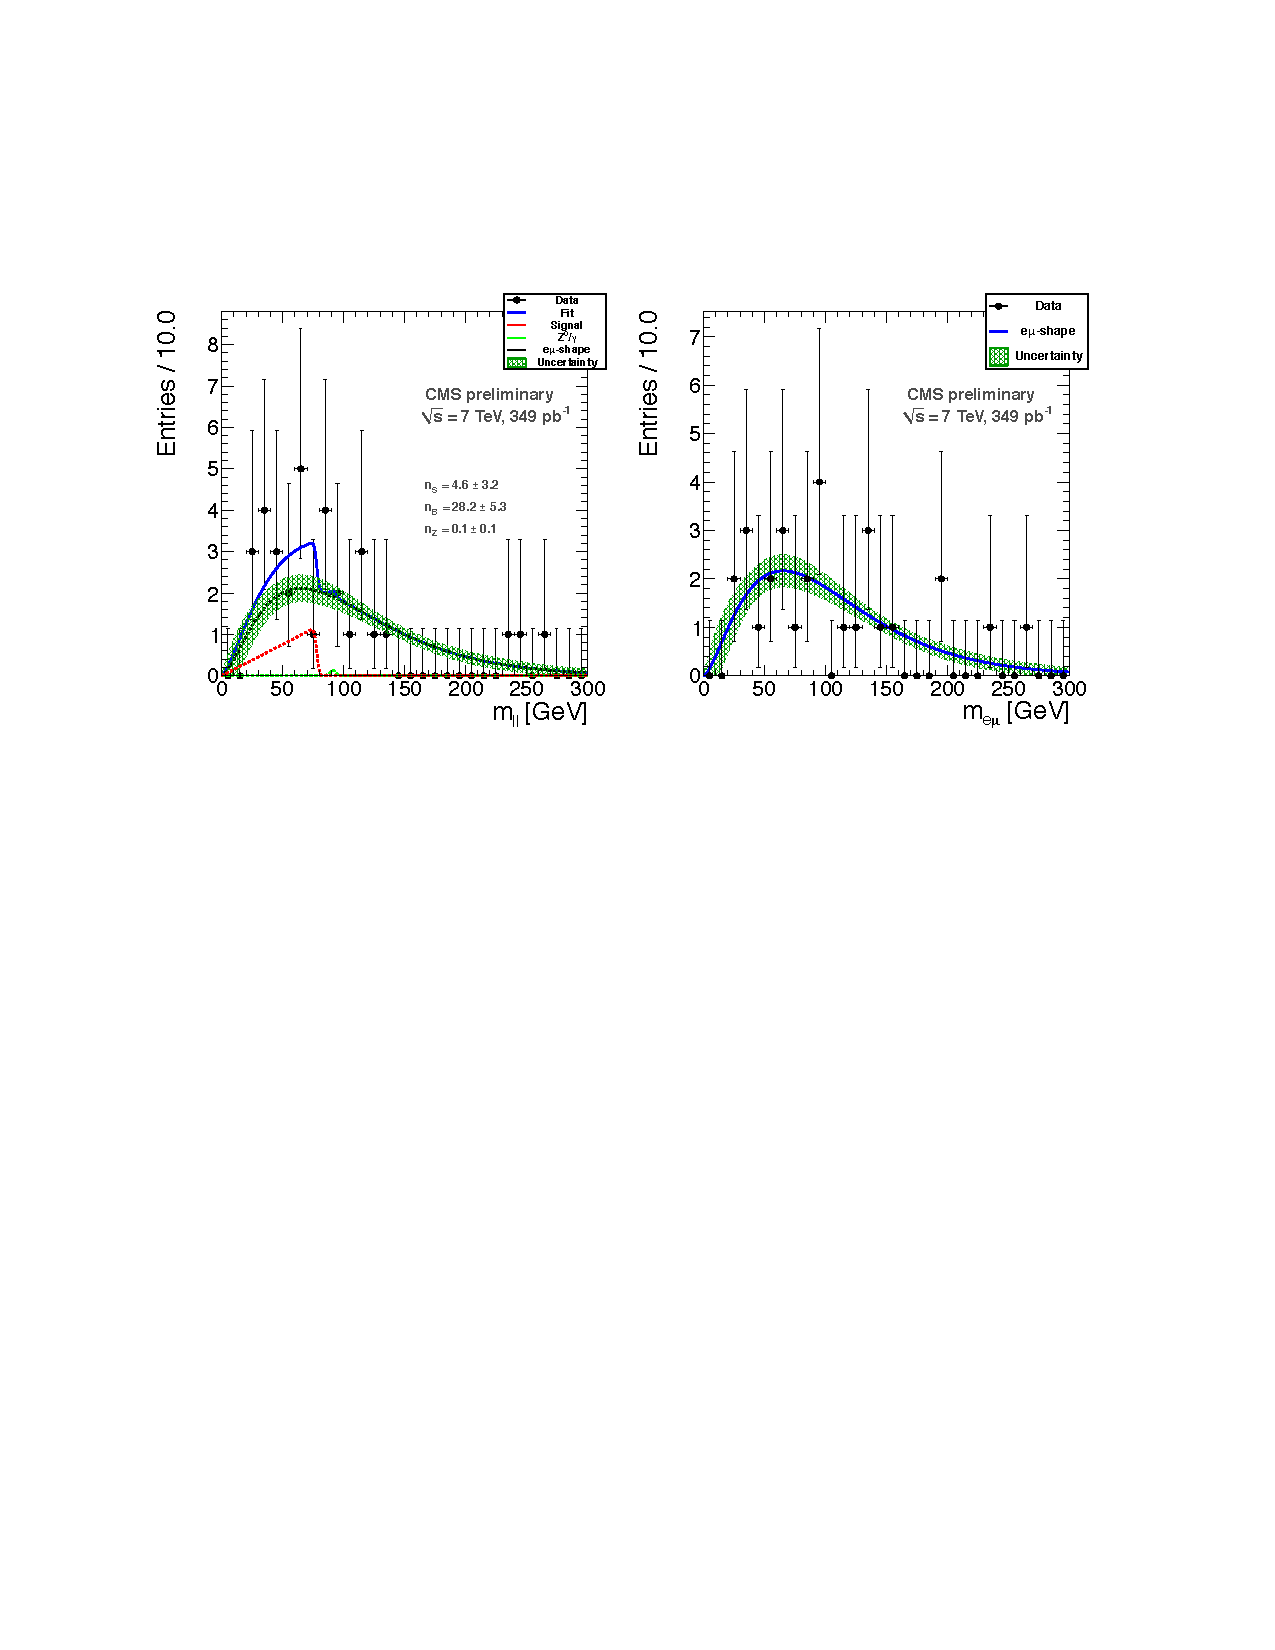
\includegraphics[width=0.75\linewidth]{plots_final/dilmass.pdf}
\caption{\label{fig:dilmass}\protect 
Results of the maximum likelihood fit to the dilepton mass distribution for events containing 
$ee$ and $\mu\mu$ lepton pairs (left) and $e\mu$ lepton pairs (right)  in the signal
region defined as \Ht\ $>$ 300~GeV, \MET\ $>$ 100 GeV.
}
\end{center}
\end{figure}

The position of the kinematic edge $M_{cut}$ is fixed based on the generator level
information for the signal model which is tested; for example, for LM1 
$M_{cut} = 78$~GeV. Finally, the $Z$ contribution is modelled by a Breit-Wigner 
convoluted with a Gaussian. We perform an extended, unbinned maximum 
likelihood (ML) fit to the distribution of dilepton mass for events containting SF lepton pairs. 
The shape of the \ttbar\ background is fixed using the results of the fit to the OF lepton pairs,
and the yield is allowed to vary within the 
statistical plus systematic uncertainty. 

We perform the fit in the control region 100 $<$ \Ht\ $<$ 300 GeV, in
which the \ttbar\ background, $Z$ background, and LM1 signal yields are allowed to vary in the fit. 
The extracted signal yield is $n_S = 2.4 \pm 4.7$, consistent with the background only 
hypothesis, as displayed in Fig.~\ref{fig:dilmasscontrol}. 
The extracted $Z$ yield is $n_Z = 4.4 \pm 4.2$, which is 
used to constrain the $Z$ yield in the signal region. 

Next, we proceed to perform the fit in the signal region \Ht\ $>$ 300 GeV. First, we
constrain the $Z$ yield in this region using an extrapolation in \Ht\ from the 
control region 100 $<$ \Ht\ $<$ 300 GeV. The $Z$ yield in the control region is
multiplied by a scale factor derived from $Z$ events in data with no requirement
on \MET, which quantifies the fraction of $Z$ events with \Ht\ $>$ 100 GeV which 
satisfy \Ht\ $>$ 300 GeV. Using this procedure we derive an upper limit on the
$Z$ yield in the signal region of $n_Z < 0.3$, which we use to constrain the
$Z$ yield in the ML fit. The extracted signal yield is $n_S = 4.6 \pm 3.2$,
which is consistent with the background only hypothesis within 1.4$\sigma$. 





